\chapter{User Interface (UI) und Interaktion}

\begin{quote}
\emph{\glqq Im Interface begegnet der Spieler dem Spiel. [...] Die Schnittstelle zwischen Mensch und Computer/Konsole etc.\grqq}~\cite[p.~161]{GameDesign} \\
\end{quote}

Das UI im Spieldesign ist fast der wichtigste Teil der Spielentwicklung, wenn man das Design des eigentlichen Spieles außen vornimmt. 
Ohne eine gute Menu führung und ein gut entworfenes User Interface ist es schwer, dass Spielerinnen und Spieler das Spiel verstehen und spielen können. 

\begin{figure}[H]
    \centering
    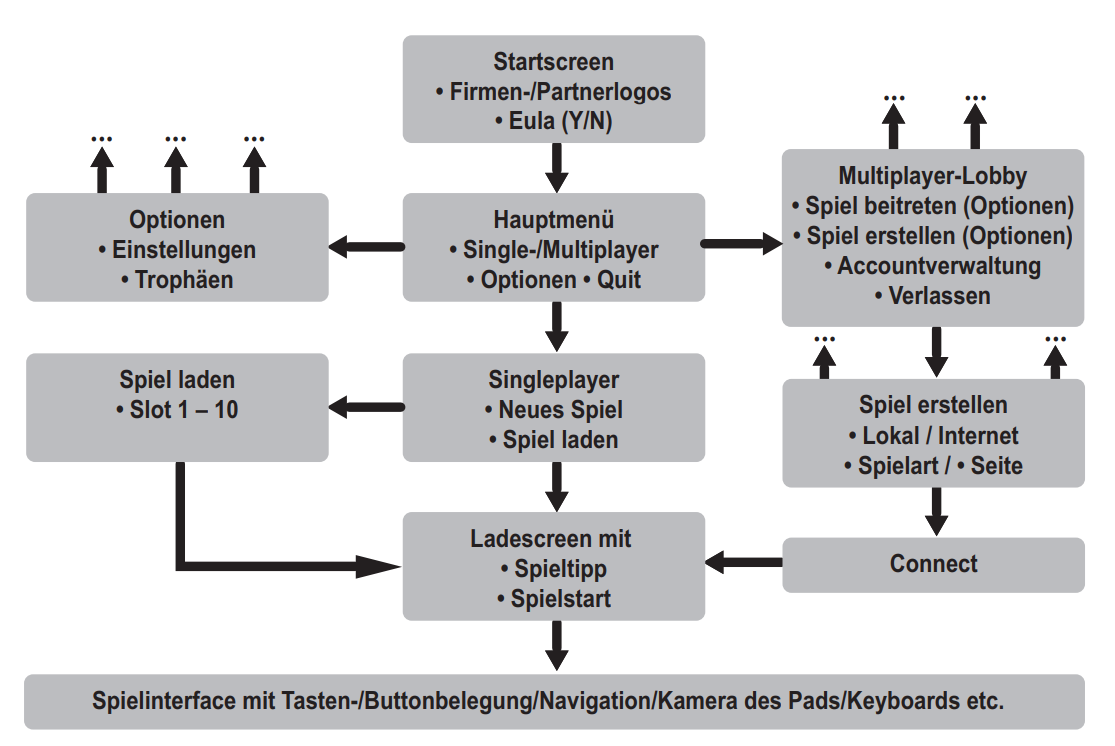
\includegraphics[width=0.8\textwidth]{chapters/03/images/Spielinterface.png}
    \caption{Ein Beispiel eines Dialogbaumes von einem Computerspiel.}
    \label{htl01}
\end{figure}

Der abgebildete Dialogbaum zeigt die verschiedenen Menüs und Screens die ein Computerspiel haben kann.
Diese unterscheiden sich in den unterschiedlichen Arten von Spielen. 
Bei einem \gls{multiplayer} Spiel soll die Möglichkeit geboten werden ein Spiel zu erstellen oder einem beizutreten. 
Während es bei einem \gls{singleplayer} wichtig ist Spielstände zu speichern und zu laden.

\pagebreak

Das \gls{UI} des Prototyps unterteilt sich in 3 verschiedene Aspekte:

\begin{itemize}
    \item Das Hauptmenü.
    \item Das \gls{UI} während des Spieles.
    \item Das Pause Menu.
\end{itemize}

\noindent
Bei der Entscheidung, welche Komplexität das User Interface des Prototyps haben soll, fiel die Wahl auf ein simples Design. 
Das \gls{UI} soll einerseits die Schlichtheit des eigentlichen Spieles wiederspiegeln und andererseits alle für das Spiel wichtigen Informationen darstellen.

\section{Gestaltung des Hauptmenüs}

Im Folgenden wird das Gestalten der Benutzeroberfläche für das Hauptmenü erläutert. 
Das Hauptmenü in der Spielentwicklung ist vergleichbar mit einem Türvorleger vor einer Haustür. Es soll das Willkommenschild für das eigentliche Spiel sein. 
Mithilfe dieses ersten Eindrucks ist es möglich zu erkennen um welche Art von Spiel es sich handelt. Das \gls{theme} des Spieles spiegelt sich in dem Design des Hintergrundes und in der Schriftart des Hauptmenüs wieder. Die Komplexität steht bei vielen Spielen in direkter Korrelation mit der Anzahl an Einstellungen in dem Hauptmenü.

\pagebreak

\subsection{Das Hauptmenü des Prototyps}

Das Hauptmenü des Prototyps besteht aus mehreren Komponenten. Die Hauptkomponente ist ein \gls{canvas}. Diesem untergeordnet ist ein Bild, ein \gls{gameObject} für das Hauptmenü und ein \gls{gameObject} für das Optionsmenü. Diese beiden GameObjecte sind die eigentlichen Menüs die dementsprechen ein- und ausgeblendet werden. Die Knöpfe die der User betätigen kann sind den Gameobjecten für das Hauptmenü und dem Optionsmenü untergeordnet. 
\subsubsection{Der Hintergrund}
Der Hintergrund des Hauptmenüs ist ein PNG von der \gls{skybox} des Spiels. 

\subsubsection{Die Buttons}
Die unten abgebildeten Abbildungen zeigen das Hauptmenü (links) und das Optionsmenü (rechts) des Prototyps. \\
In dem Hauptmenü gibt es drei verschiedene Buttons: Play, Options and Quit.\\
Play startet den Spielablauf, Options öffnet das Optionsmenü und Quit schließt das Spiel.\\\\

In dem Optionsmenü befindet sich die Lautstärkenregelung und... und der Back Button um zurück in das Hauptmenü zu kommen.
    


\begin{figure}[H]
    \centering
    \begin{minipage}{0.4\textwidth}
        \centering
        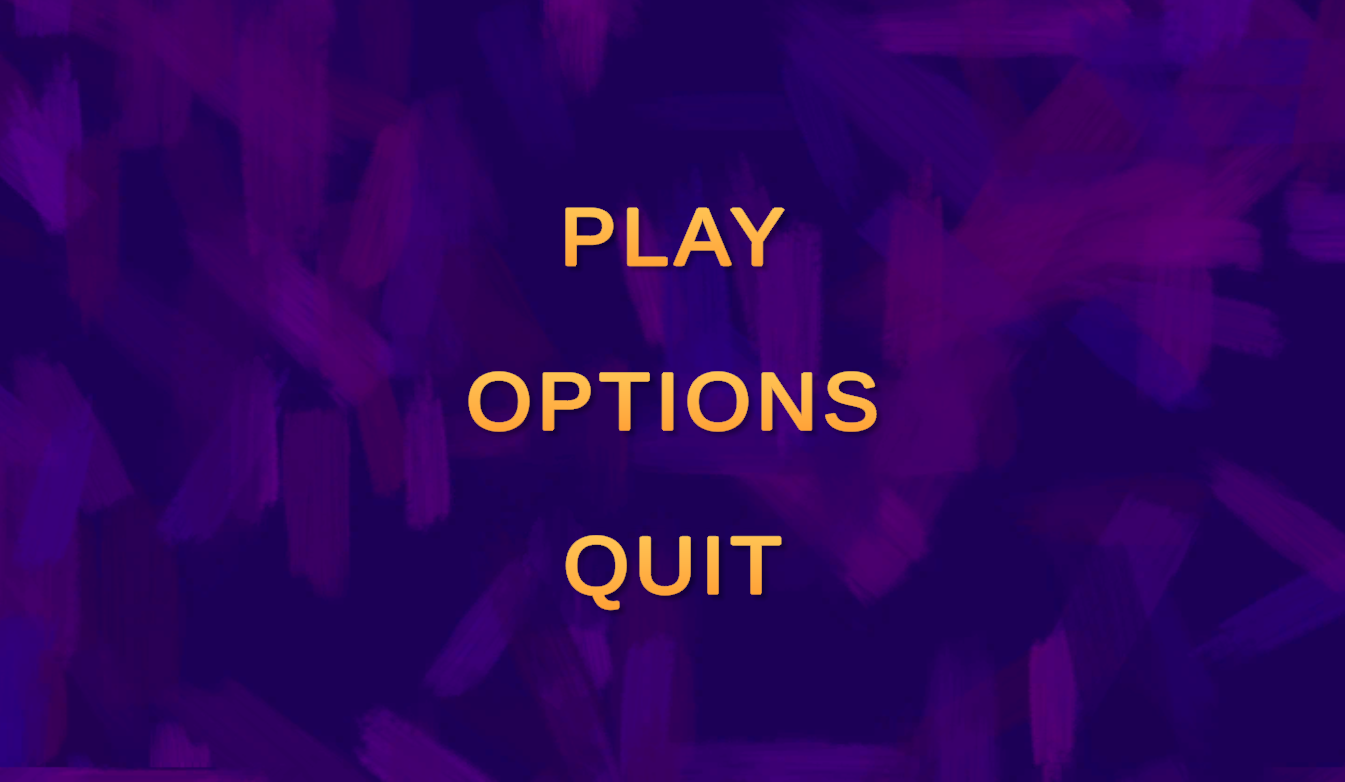
\includegraphics[width=\linewidth]{chapters/03/images/MainMenu.png}
        \caption{Das Hauptmenü des Prototyps.}
        \label{htl02a}
    \end{minipage}%
    \hspace{1cm}% Adjust the space here as needed
    \begin{minipage}{0.4\textwidth}
        \centering
        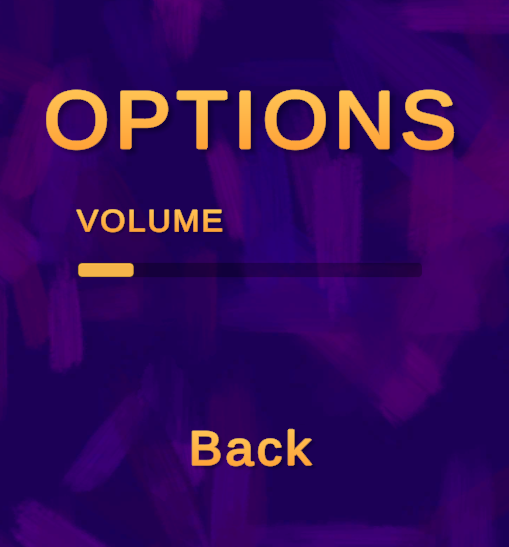
\includegraphics[width=\linewidth]{chapters/03/images/OptionsMainMenu.png}
        \caption{Das Optionsmenü des Prototyps.}
        \label{htl02b}
    \end{minipage}
\end{figure}



\section{Game UI und Spielmechanik-Anzeigen}

\begin{figure}[H]
    \centering
    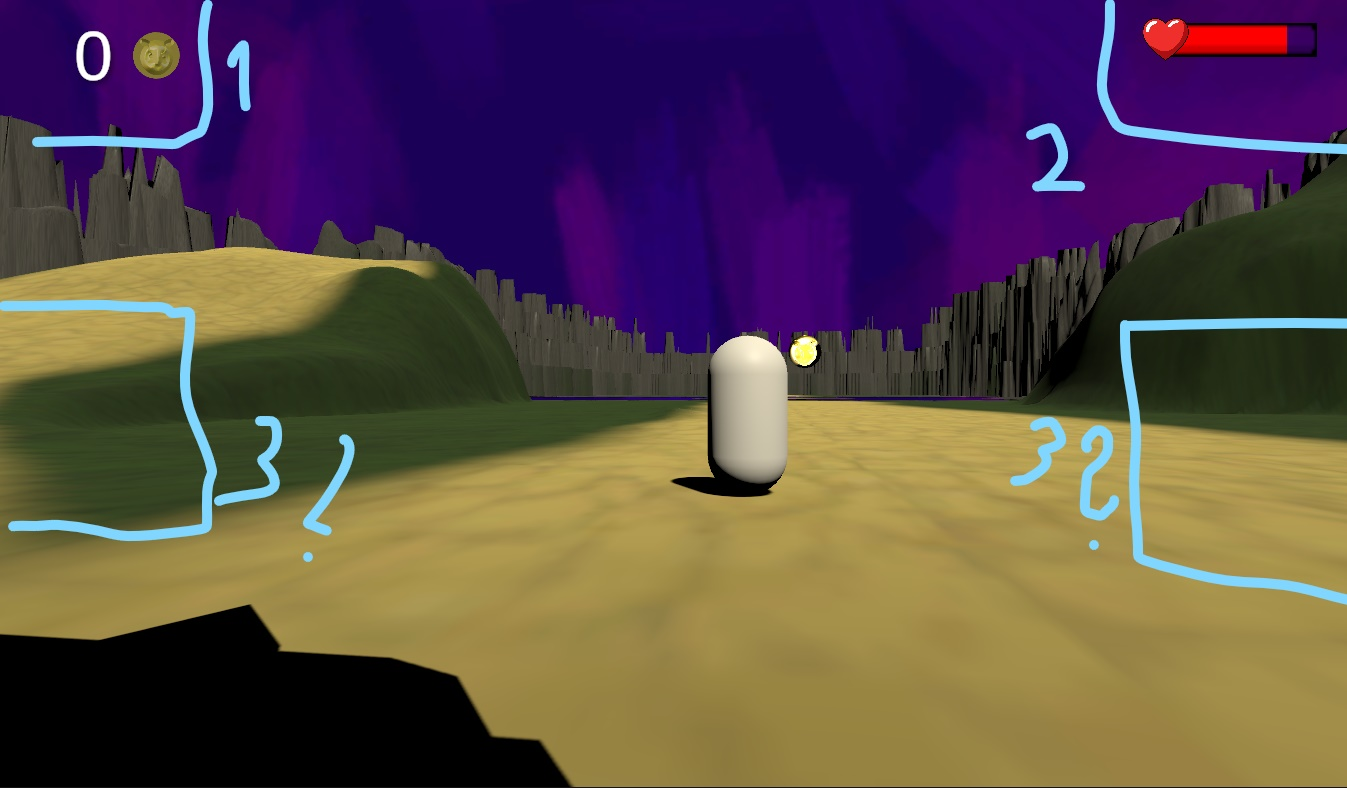
\includegraphics[width=1\textwidth]{chapters/03/images/InkedGameUI.jpg}
    \caption{Das UI während des Spiels.}
    \label{htl03}
\end{figure}

\section{Optionen und Einstellungen}
\section{Pause-Funktion und Benutzerfreundlichkeit}